\documentclass[journal, a4paper]{IEEEtran}

% some very useful LaTeX packages include:

%\usepackage{cite}      % Written by Donald Arseneau
                        % V1.6 and later of IEEEtran pre-defines the format
                        % of the cite.sty package \cite{} output to follow
                        % that of IEEE. Loading the cite package will
                        % result in citation numbers being automatically
                        % sorted and properly "ranged". i.e.,
                        % [1], [9], [2], [7], [5], [6]
                        % (without using cite.sty)
                        % will become:
                        % [1], [2], [5]--[7], [9] (using cite.sty)
                        % cite.sty's \cite will automatically add leading
                        % space, if needed. Use cite.sty's noadjust option
                        % (cite.sty V3.8 and later) if you want to turn this
                        % off. cite.sty is already installed on most LaTeX
                        % systems. The latest version can be obtained at:
                        % http://www.ctan.org/tex-archive/macros/latex/contrib/supported/cite/

\usepackage{graphicx}   % Written by David Carlisle and Sebastian Rahtz
                        % Required if you want graphics, photos, etc.
                        % graphicx.sty is already installed on most LaTeX
                        % systems. The latest version and documentation can
                        % be obtained at:
                        % http://www.ctan.org/tex-archive/macros/latex/required/graphics/
                        % Another good source of documentation is "Using
                        % Imported Graphics in LaTeX2e" by Keith Reckdahl
                        % which can be found as esplatex.ps and epslatex.pdf
                        % at: http://www.ctan.org/tex-archive/info/

%\usepackage{psfrag}    % Written by Craig Barratt, Michael C. Grant,
                        % and David Carlisle
                        % This package allows you to substitute LaTeX
                        % commands for text in imported EPS graphic files.
                        % In this way, LaTeX symbols can be placed into
                        % graphics that have been generated by other
                        % applications. You must use latex->dvips->ps2pdf
                        % workflow (not direct pdf output from pdflatex) if
                        % you wish to use this capability because it works
                        % via some PostScript tricks. Alternatively, the
                        % graphics could be processed as separate files via
                        % psfrag and dvips, then converted to PDF for
                        % inclusion in the main file which uses pdflatex.
                        % Docs are in "The PSfrag System" by Michael C. Grant
                        % and David Carlisle. There is also some information
                        % about using psfrag in "Using Imported Graphics in
                        % LaTeX2e" by Keith Reckdahl which documents the
                        % graphicx package (see above). The psfrag package
                        % and documentation can be obtained at:
                        % http://www.ctan.org/tex-archive/macros/latex/contrib/supported/psfrag/

\usepackage{subfigure} % Written by Steven Douglas Cochran
                        % This package makes it easy to put subfigures
                        % in your figures. i.e., "figure 1a and 1b"
                        % Docs are in "Using Imported Graphics in LaTeX2e"
                        % by Keith Reckdahl which also documents the graphicx
                        % package (see above). subfigure.sty is already
                        % installed on most LaTeX systems. The latest version
                        % and documentation can be obtained at:
                        % http://www.ctan.org/tex-archive/macros/latex/contrib/supported/subfigure/

\usepackage{url}        % Written by Donald Arseneau
                        % Provides better support for handling and breaking
                        % URLs. url.sty is already installed on most LaTeX
                        % systems. The latest version can be obtained at:
                        % http://www.ctan.org/tex-archive/macros/latex/contrib/other/misc/
                        % Read the url.sty source comments for usage information.

%\usepackage{stfloats}  % Written by Sigitas Tolusis
                        % Gives LaTeX2e the ability to do double column
                        % floats at the bottom of the page as well as the top.
                        % (e.g., "\begin{figure*}[!b]" is not normally
                        % possible in LaTeX2e). This is an invasive package
                        % which rewrites many portions of the LaTeX2e output
                        % routines. It may not work with other packages that
                        % modify the LaTeX2e output routine and/or with other
                        % versions of LaTeX. The latest version and
                        % documentation can be obtained at:
                        % http://www.ctan.org/tex-archive/macros/latex/contrib/supported/sttools/
                        % Documentation is contained in the stfloats.sty
                        % comments as well as in the presfull.pdf file.
                        % Do not use the stfloats baselinefloat ability as
                        % IEEE does not allow \baselineskip to stretch.
                        % Authors submitting work to the IEEE should note
                        % that IEEE rarely uses double column equations and
                        % that authors should try to avoid such use.
                        % Do not be tempted to use the cuted.sty or
                        % midfloat.sty package (by the same author) as IEEE
                        % does not format its papers in such ways.

\usepackage{amsmath}    % From the American Mathematical Society
                        % A popular package that provides many helpful commands
                        % for dealing with mathematics. Note that the AMSmath
                        % package sets \interdisplaylinepenalty to 10000 thus
                        % preventing page breaks from occurring within multiline
                        % equations. Use:
%\interdisplaylinepenalty=2500
                        % after loading amsmath to restore such page breaks
                        % as IEEEtran.cls normally does. amsmath.sty is already
                        % installed on most LaTeX systems. The latest version
                        % and documentation can be obtained at:
                        % http://www.ctan.org/tex-archive/macros/latex/required/amslatex/math/

\usepackage{mathbbol}
\makeatletter
\newif\if@restonecol
\makeatother
\let\algorithm\relax
\let\endalgorithm\relax
\usepackage[linesnumbered,ruled,vlined]{algorithm2e}%[ruled,vlined]{
\usepackage{algpseudocode}
\usepackage{amsmath}
\renewcommand{\algorithmicrequire}{\textbf{Input:}}  % Use Input in the format of Algorithm
\renewcommand{\algorithmicensure}{\textbf{Output:}} % Use Output in the format of Algorithm 
% Other popular packages for formatting tables and equations include:

%\usepackage{array}
% Frank Mittelbach's and David Carlisle's array.sty which improves the
% LaTeX2e array and tabular environments to provide better appearances and
% additional user controls. array.sty is already installed on most systems.
% The latest version and documentation can be obtained at:
% http://www.ctan.org/tex-archive/macros/latex/required/tools/

% V1.6 of IEEEtran contains the IEEEeqnarray family of commands that can
% be used to generate multiline equations as well as matrices, tables, etc.

% Also of notable interest:
% Scott Pakin's eqparbox package for creating (automatically sized) equal
% width boxes. Available:
% http://www.ctan.org/tex-archive/macros/latex/contrib/supported/eqparbox/

% *** Do not adjust lengths that control margins, column widths, etc. ***
% *** Do not use packages that alter fonts (such as pslatex).         ***
% There should be no need to do such things with IEEEtran.cls V1.6 and later.


% Your document starts here!
\begin{document}
\begin{titlepage}

\newcommand{\HRule}{\rule{\linewidth}{0.5mm}} % Defines a new command for the horizontal lines, change thickness here

\center % Center everything on the page
 %----------------------------------------------------------------------------------------
%	LOGO SECTION
%----------------------------------------------------------------------------------------

~\\[1cm]

\includegraphics{SCUT.png}\\[2cm] % Include a department/university logo - this will require the graphicx package

%----------------------------------------------------------------------------------------
%	TITLE SECTION
%----------------------------------------------------------------------------------------

\HRule \\[1cm]
{ \huge \bfseries The Experiment Report of \textit{Machine Learning} }\\[0.6cm] % Title of your document
\HRule \\[2cm]
%----------------------------------------------------------------------------------------
%	HEADING SECTIONS
%----------------------------------------------------------------------------------------


\textsc{\LARGE \textbf{School:} School of Software Engineering}\\[1cm]
\textsc{\LARGE \textbf{Subject:} Software Engineering}\\[2cm] 

 
%----------------------------------------------------------------------------------------
%	AUTHOR SECTION
%----------------------------------------------------------------------------------------

\begin{minipage}{0.4\textwidth}
\begin{flushleft} \large
\emph{Author:}\\
Lizhao Liu % Your name
\end{flushleft}
\end{minipage}
~
\begin{minipage}{0.4\textwidth}
\begin{flushright} \large
\emph{Supervisor:} \\
Mingkui Tan % Supervisor's Name
\end{flushright}
\end{minipage}\\[2cm]
~
\begin{minipage}{0.4\textwidth}
\begin{flushleft} \large
\emph{Student ID:}\\
201730683109
\end{flushleft}
\end{minipage}
~
\begin{minipage}{0.4\textwidth}
\begin{flushright} \large
\emph{Grade:} \\
Undergraduate
\end{flushright}
\end{minipage}\\[2cm]

% If you don't want a supervisor, uncomment the two lines below and remove the section above
%\Large \emph{Author:}\\
%John \textsc{Smith}\\[3cm] % Your name

%----------------------------------------------------------------------------------------
%	DATE SECTION
%----------------------------------------------------------------------------------------

{\large \today}\\[2cm] % Date, change the \today to a set date if you want to be precise

 
%----------------------------------------------------------------------------------------

\vfill % Fill the rest of the page with whitespace

\end{titlepage}

% Define document title and author
	\title{Adaboost for face image classification}
	\maketitle

% Write abstract here
\begin{abstract}
In this report, we solve the face/non-face classification problem by adaboost with Decision Tree Classifier (DTC) as weak learner. \\
We perform experiments on three aspects: \\
1. Weak learner's performance effect. \\
2. Number of weak learner's exploration. \\
\end{abstract}

% Each section begins with a \section{title} command
\section{Introduction}
	% \PARstart{}{} creates a tall first letter for this first paragraph
\PARstart{A}{daboost} short for "Adaptive Boosting",  is an ensemble method that combine a bunch of weak learners into a strong learner which outperforms all the weak learners. It's wildly used in academic and industry community, which make it very important for us to fully explore it. We will explore the the effect of weak learner's performance and the performance with different number of weak learner. 

% Main Part
\section{Methods and Theory}
In this part, we define Adaboost algorithm.
\subsection{Adaboost}
Given dataset $ D=\{x_{i}, y_{i}\}_{i=1}^{m}$, where $x_{i} \in \mathbf{R}^{n}$. $y_{i} \in \{-1, 1\}$ and weak Learner $L(x) \in \{-1, 1\} $, Adaboost algorithm can be found in Algorithm~\ref{alg:adaboost}. \par

\begin{algorithm}
	\label{alg:adaboost}
	\caption{Adaboost}
	\KwIn{Training Dataset $ D=\{x_{i}, y_{i}\}_{i=1}^{m}$, num weak learner $N$, weak learner $L$}
	\KwOut{Final learner $H(x)$}
	$w_1(i) \gets \frac{1}{m}$ where i = 1, 2, ..., m \\
	\For{$idx = 1, 2, ..., N$}
	{
		$h_{idx}(x) = L(D, w_{idx})$ \\
		$\epsilon_{idx} = \Sigma_{i=1}^m w_{idx}(i) \mathbb{1}(h_{idx}(x_i) \neq y_i) $ \\
		$\alpha_{idx} = \frac{1}{2} \log{\frac{1 - \epsilon_{idx}}{\epsilon_{idx}}}$ \\
		$w_{idx+1}(i) = w_{idx}(i) * exp(-1 * \alpha_{idx} * y_i * h_{idx}(x_i))$ where i = 1, 2, .., m \\
		$w_{idx+1} = \frac{w_{idx+1}}{\Sigma_{i=1}^m w_{idx}(i)}  $ \\
	}
	return $H(x) = \Sigma_{idx=1}^N \alpha_{idx} h_{idx}(x)$
\end{algorithm} \par

We can see that, in each iteration, the examples that correctly classified by previous weak learner, will get a smaller weight, so that current learner can pay more attention to the misclassified examples. 


\section{Experiments}
\subsection{Dataset}
We conduct all the experiments on self constructed face/non-face dataset, which has 500 256x256 face images and 500 32x32 non-face images. All images have 3 channels. We preprocess all the images into 24x24 gray scale images. We then convert them by using NPD features. Finally, each example's form is $(x, y)$, where $x \in \mathbf{R}^{165600}$ and $y \in \{-1, +1\}$, where $+1$ means face and $-1$ means non-face. We randomly split the dataset into three part: 700 training examples, 100 validation examples and 200 test examples. $X_{train},~X_{val}~and~X_{test} $ are divided by 256 for scale purporse.

\subsection{Implementation}
We implement the Adaboost using python and mainly rely on the numpy package.

\subsection{Weak learner's performance's effect.}
In this section, we explore the influence of weak learner's performance in Adaboost. \par 
We first explore the performance of DTC under different depths setting. From Fig~\ref{fig:d_weak_acc} we can see that, as the depth of DTC goes depper, its performance on training set become better but in validation set, the performance of it first gets better and then goes down which indicating the overfitting problem. The best performance in validation set is $89$ occurs when $depth = 4$. \par
Then we explore Adaboost's performance with different weaker learner.  We set number of weak learner to five due to computation limitation. We can see from Fig~\ref{fig:d_acc} that, both Adaboost and DTC suffer from overfitting prolem. But Adaboost outperform DTC under all setting except in validation set when depth equals to 5. We can see that, as the performance of weak learner goes up, the performance of Adaboost goes down, maybe due to the overfitting problem. The intuition is that, if a weak learner's performance is good enough in training set, then Adaboost with more weak learner is prone to overfit the dataset.  \par

\begin{figure}[!hbt]
	% Center the figure.
	\begin{center}
		% Include the eps file, scale it such that it's width equals the column width. You can also put width=8cm for example...
		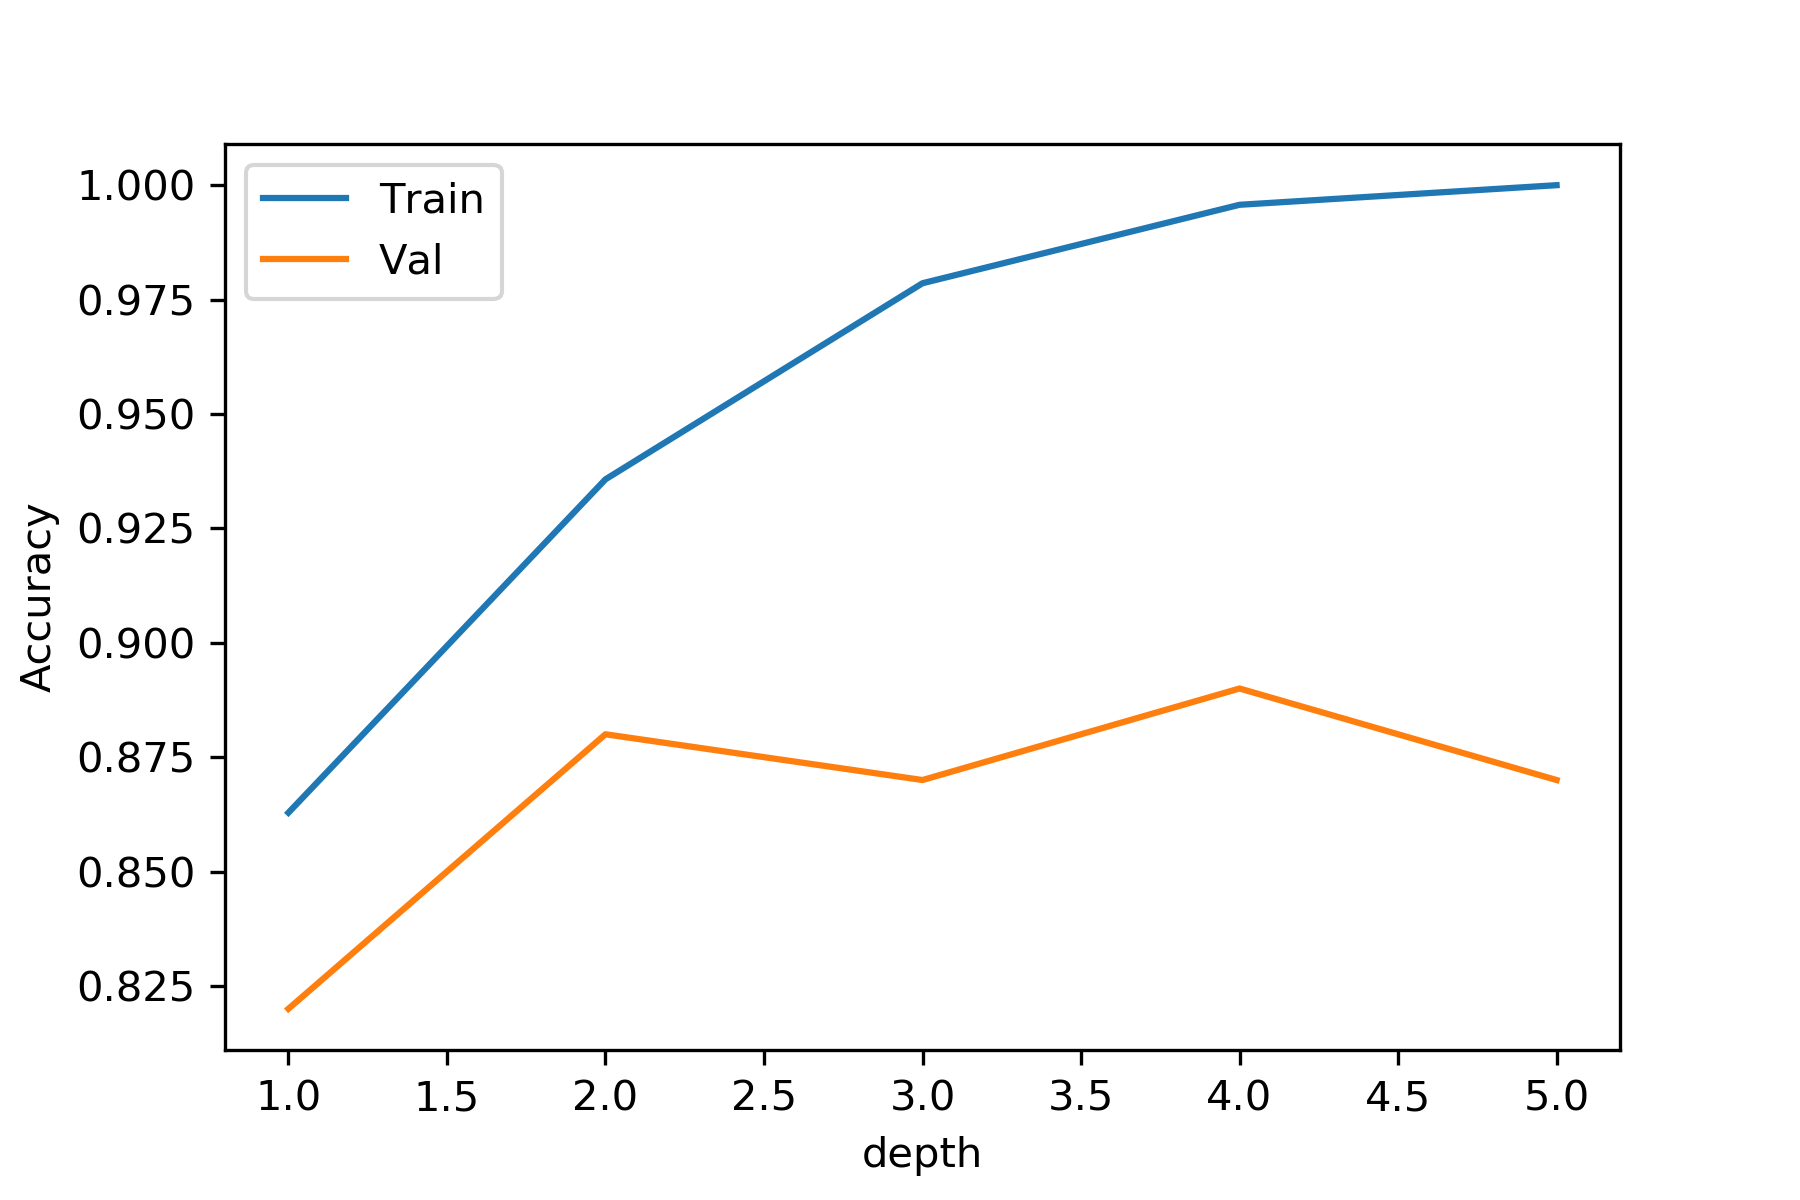
\includegraphics[width=\columnwidth]{d_weak_acc}
		% Create a subtitle for the figure.
		\caption{DTC accuracy under different $depth$.}
		% Define the label of the figure. It's good to use 'fig:title', so you know that the label belongs to a figure.
		\label{fig:d_weak_acc}
	\end{center}
\end{figure} \par

\begin{figure}[!hbt]
	% Center the figure.
	\begin{center}
		% Include the eps file, scale it such that it's width equals the column width. You can also put width=8cm for example...
		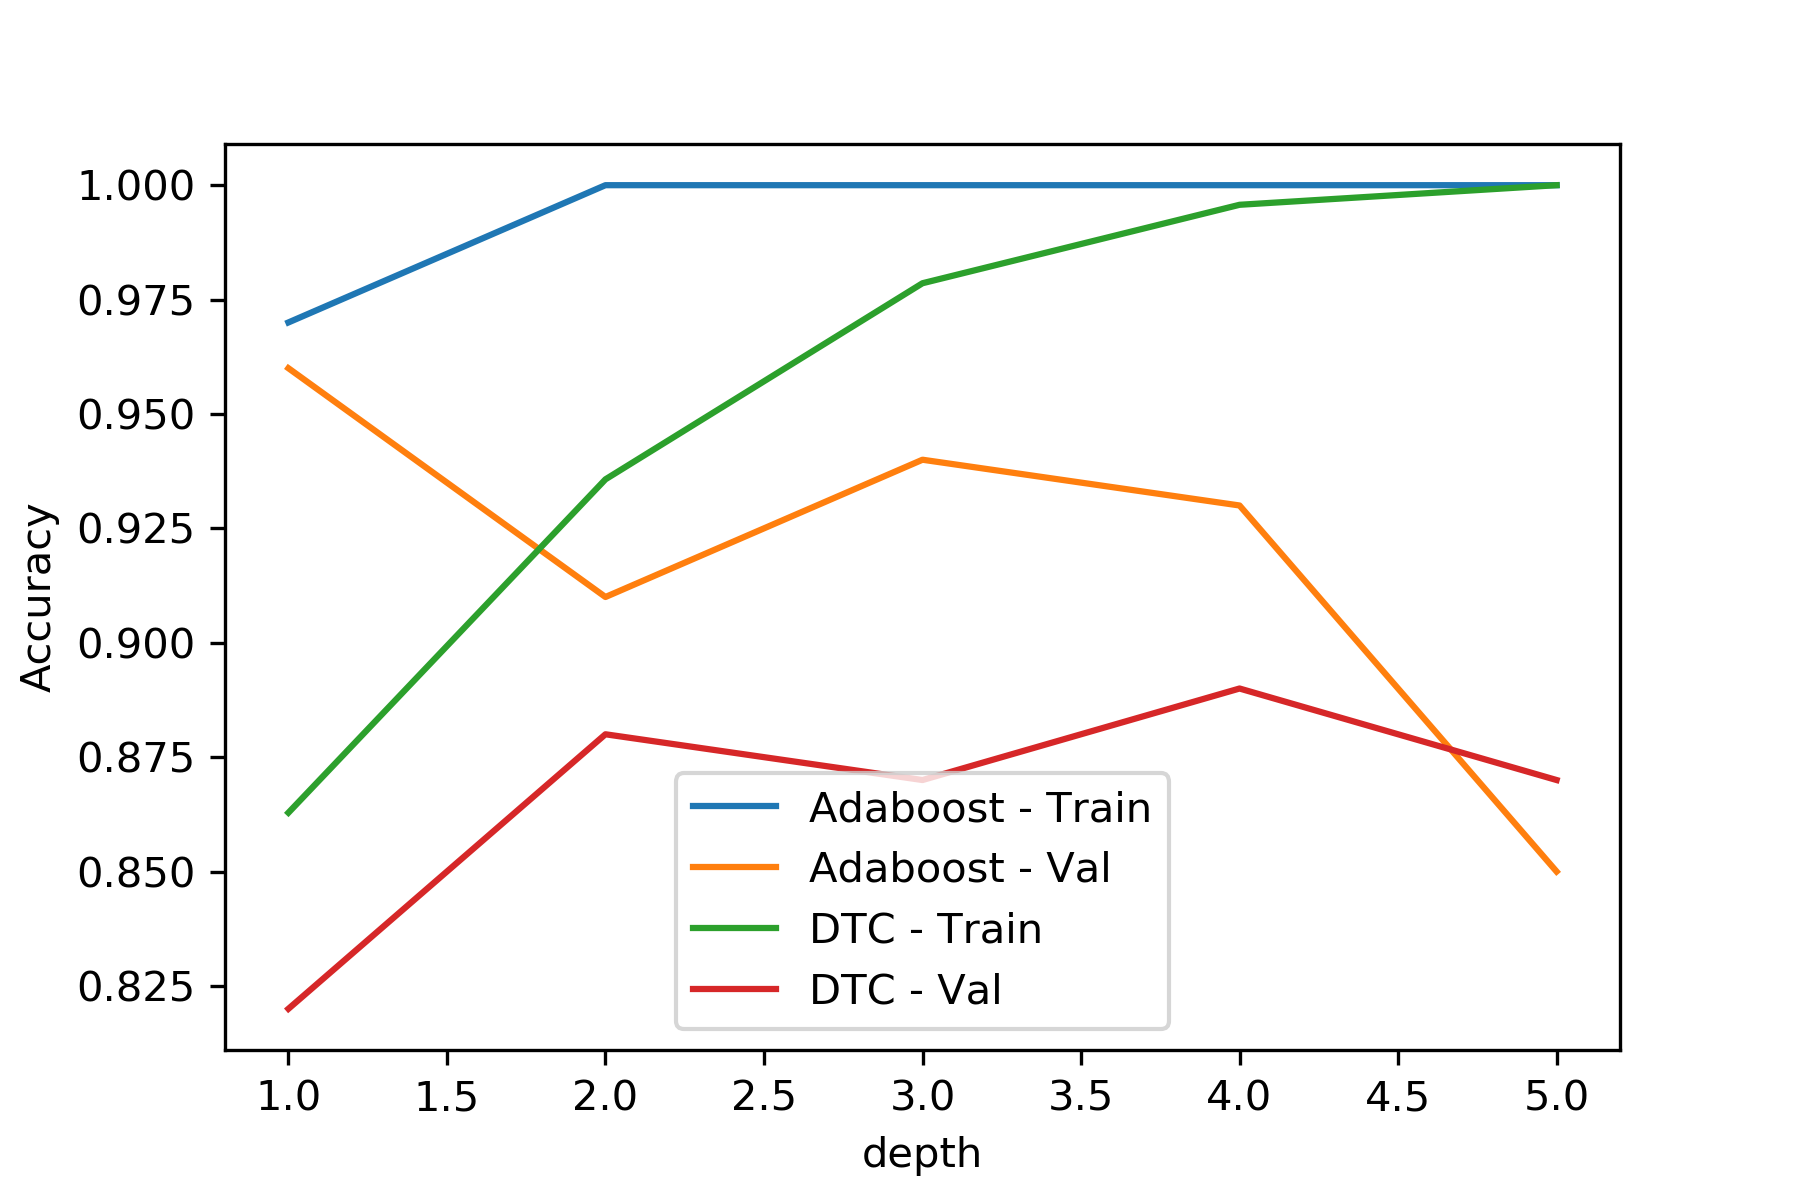
\includegraphics[width=\columnwidth]{d_acc}
		% Create a subtitle for the figure.
		\caption{Adaboost and DTC accuracy under different $depth$. Note that we set number of weak learner to 5 in Adaboost.}
		% Define the label of the figure. It's good to use 'fig:title', so you know that the label belongs to a figure.
		\label{fig:d_acc}
	\end{center}
\end{figure} \par

\begin{table}[!hbt]
	% Center the table
	\begin{center}
		% Title of the table
		\caption{DTC and Adaboost accuracy on validation set. Best result are in bold.}
		\label{tab:d_dtc_ad}
		% Table itself: here we have two columns which are centered and have lines to the left, right and in the middle: |c|c|
		\begin{tabular}{|c|c|c|c|c|c|}
			\hline
			$depth$  & 1 & 2 & 3 & 4 & 5 \\
			\hline
			$DTC$   & 0.82 & 0.88 & 0.87 & \textbf{0.89} & 0.87   \\
			\hline
			$Adaboost$  & \textbf{0.96} & 0.91 & 0.94 & 0.93 & 0.85 \\
			\hline
		\end{tabular}
	\end{center}
\end{table} \par

\subsection{Performance}
Now we report the final performance of Adaboost under the best settings e.g. DTC'depth = 3 and number of weak learner = 5. The final result is shown in Fig~\ref{tab:final_performance}.

\begin{table}[!hbt]
	% Center the table
	\begin{center}
		% Title of the table
		\caption{Adaboost's best accuracy. }
		\label{tab:final_performance}
		% Table itself: here we have two columns which are centered and have lines to the left, right and in the middle: |c|c|
		\begin{tabular}{|c|c|c|}
			\hline
			$train$  & $validation$ & $test$  \\
			\hline
			1.00   & 0.98 & 0.97  \\
			\hline
		\end{tabular}
	\end{center}
\end{table} \par

\subsection{Number of weak learner's exploration}
In this section, we conduct experiment on number of weak learner's exploration. \par 
We first set the depth to 1 due to computation limitation. Under this setting, More weak Learner benefits the Adaboost, as shown in Fig~\ref{fig:n_ad_acc}.\par
Then we evalutate the performance of Adaboost under settings that DTC' depth ranges from 1 to 5 and number of weak learner ranges from 1 to 5. As illustrated in Fig~\ref{fig:dn_ad_tr_acc}, in training set, Adaboost benefits from both the depth and the number of weak learners. Note that, as the depth of weak learner goes up, the performance gained by adaboost goes down. As shown in Fig~\ref{fig:dn_ad_val_acc}, when DTC's depth equals to 3, as the number of weak learner goes up, Adaboost has better performance. When DTC's depth equals to 5, Adaboost's performance is the worst. \par
Now, we cann draw the following conclusions: \\
1. Weaker learner gets larger performance gain in Adaboost. \\
2. Very Strong weak learner tends to have overfitting problem in Adaboost. \\
3. More weak learner boost the performance in Adaboost when weak learner is not very strong. \par

\begin{figure}[!hbt]
	% Center the figure.
	\begin{center}
		% Include the eps file, scale it such that it's width equals the column width. You can also put width=8cm for example...
		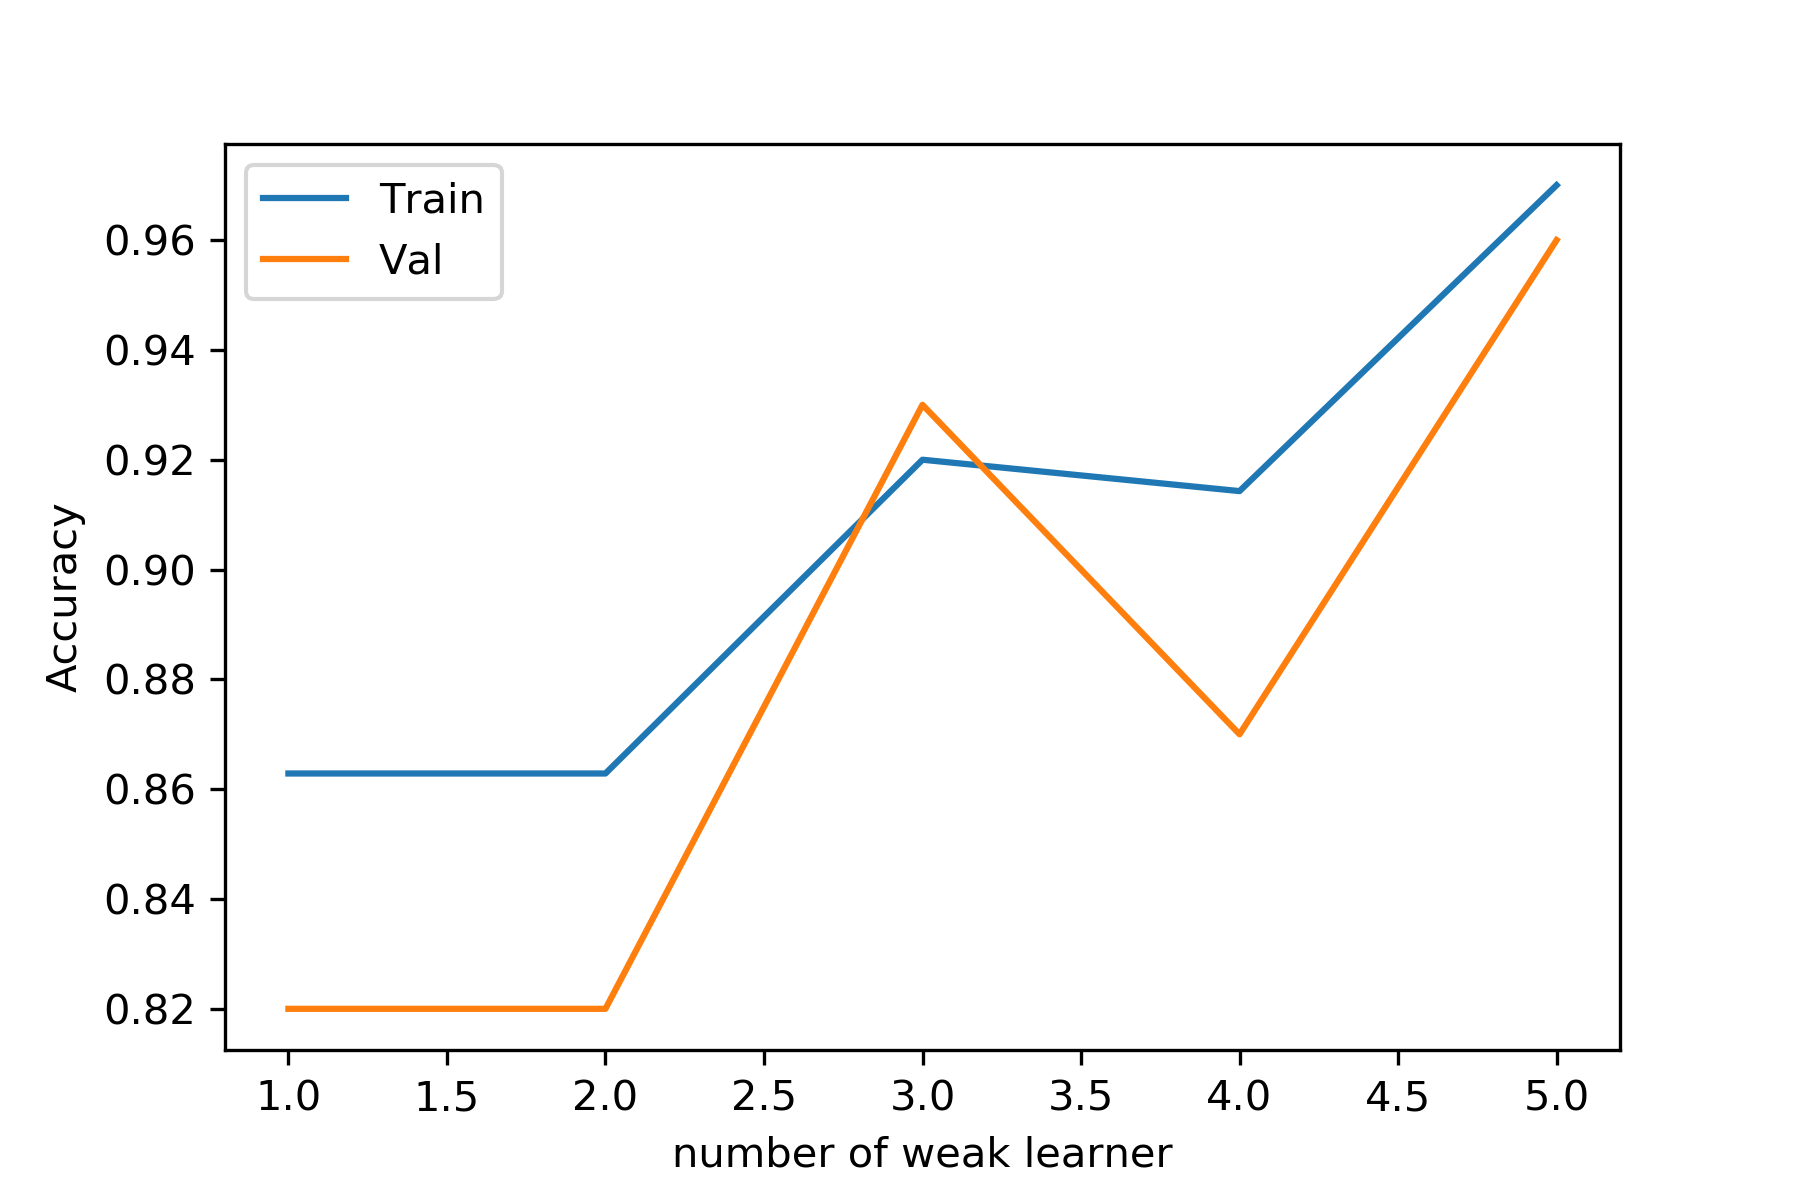
\includegraphics[width=\columnwidth]{n_ad_acc}
		% Create a subtitle for the figure.
		\caption{Adaboost accuracy with different number of DTC ($depth=1$).}
		% Define the label of the figure. It's good to use 'fig:title', so you know that the label belongs to a figure.
		\label{fig:n_ad_acc}
	\end{center}
\end{figure} \par

\begin{figure}[!hbt]
	% Center the figure.
	\begin{center}
		% Include the eps file, scale it such that it's width equals the column width. You can also put width=8cm for example...
		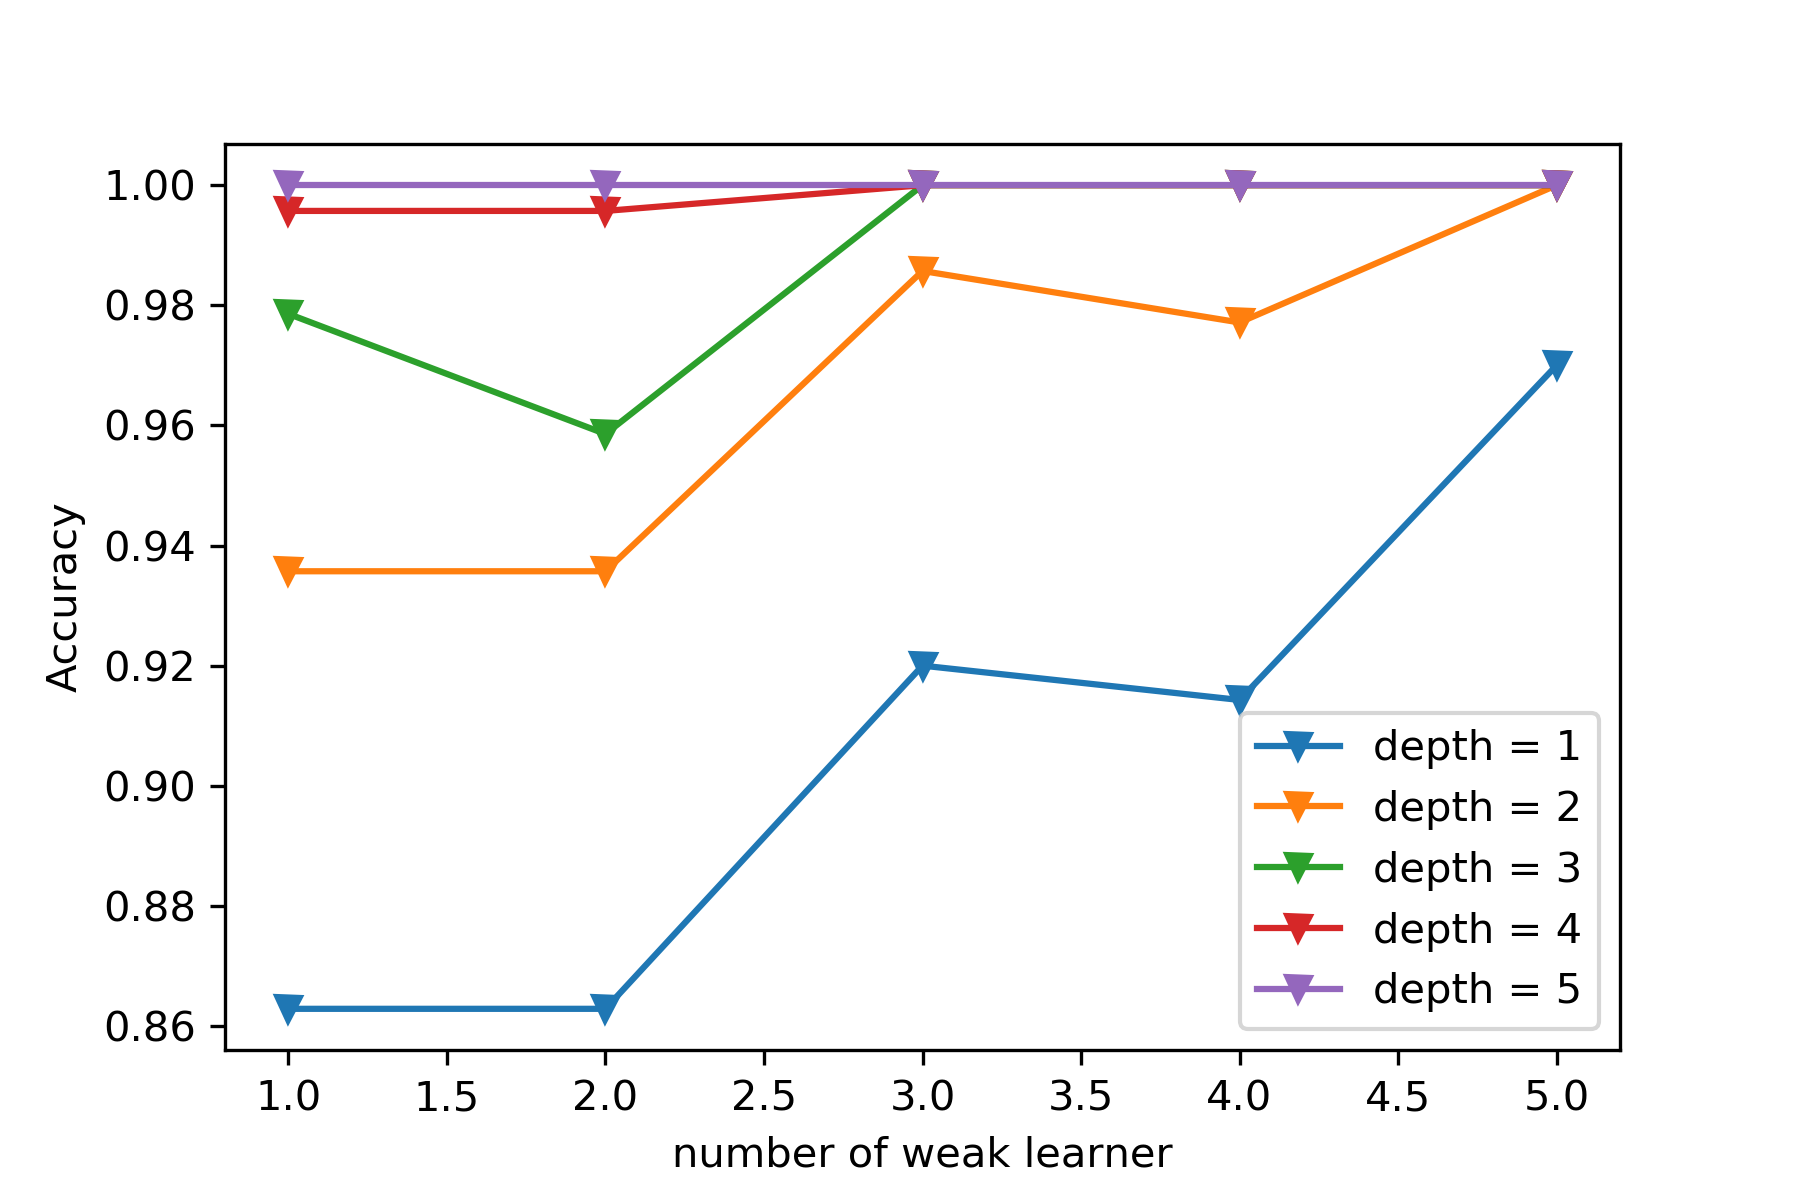
\includegraphics[width=\columnwidth]{dn_ad_tr_acc}
		% Create a subtitle for the figure.
		\caption{Adaboost accuracy with different number of DTC ($depth = 1, 2, 3, 4, 5$) in training set.}
		% Define the label of the figure. It's good to use 'fig:title', so you know that the label belongs to a figure.
		\label{fig:dn_ad_tr_acc}
	\end{center}
\end{figure} \par

\begin{figure}[!hbt]
	% Center the figure.
	\begin{center}
		% Include the eps file, scale it such that it's width equals the column width. You can also put width=8cm for example...
		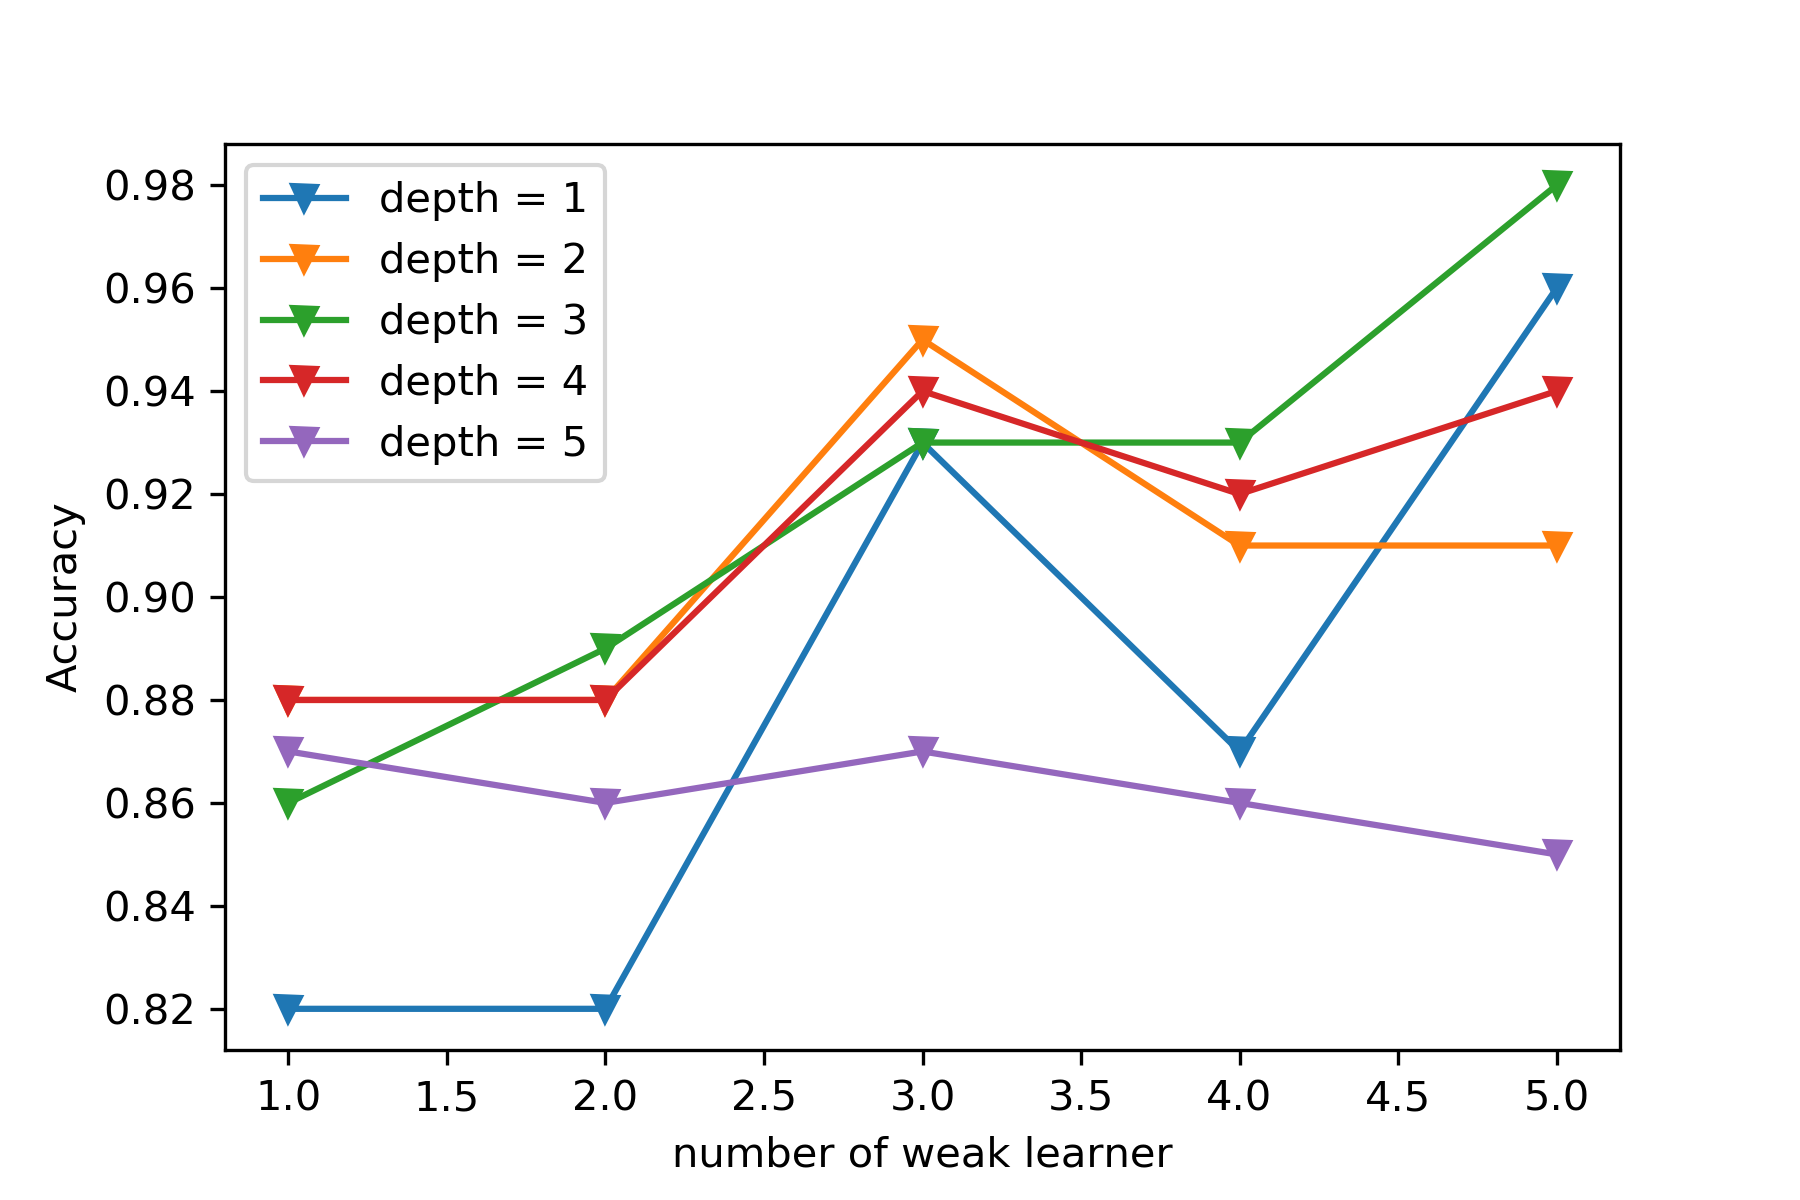
\includegraphics[width=\columnwidth]{dn_ad_val_acc}
		% Create a subtitle for the figure.
		\caption{Adaboost accuracy with different number of DTC ($depth = 1, 2, 3, 4, 5$) in validation set.}
		% Define the label of the figure. It's good to use 'fig:title', so you know that the label belongs to a figure.
		\label{fig:dn_ad_val_acc}
	\end{center}
\end{figure} \par

\section{Conclusion}
In this report, we explore Adaboost algorithm. Specifically, we explore the weak learner's performance and number of weak learner in Adaboost. We draw the conclusions that weaker learner can get more performance gain in Adaboost and stronger learner tends to have overfitting problem in Adaboost. And finally we report the performance on test set under the best validation setting. \par


% Your document ends here!


\end{document}